\documentclass[AutoFakeBold,AutoFakeSlant]{beamer}
\usepackage{ctex}
\usepackage{hyperref}
\usepackage[defaultsans]{droidsans}
\usepackage{fontspec}
\usepackage{newtxmath}
\usepackage{latexsym,amsmath,xcolor,multicol,booktabs,calligra}
\usepackage{graphicx,tabularx,multirow,makecell}
\usepackage{tikz}
\usetikzlibrary{arrows.meta,positioning}
\usetheme{Madrid}
\usecolortheme{default}
\setbeamertemplate{navigation symbols}{}
\setbeamertemplate{footline}[frame number]
\graphicspath{{./figures_lab4_23/}}

% 代码/路径/符号安全排版（避免 < > " [ ] | 等在 PDF 中失真）
\usepackage{textcomp}
\newcommand{\sepbar}{\quad\textbar\quad}
\newcommand{\arrown}{\ensuremath{\rightarrow}}

\author{李禹江，张博涵，蒋兴宇}
\title{Android 隐私检测系统\\Lab4-2 / Lab4-3 动态验证实验汇报}
\subtitle{Frida 三层 Hook \textbullet\ mitm 网络主轨 \textbullet\ Lab4-2/3 十五 App 实验}
\institute{我的刀盾队}
\date{2026-06-12}

\begin{document}
\kaishu

\begin{frame}
    \titlepage
\end{frame}

\begin{frame}
    \frametitle{目录}
    \tableofcontents
\end{frame}

\section{实验背景与范围}

\begin{frame}
    \frametitle{汇报范围}
    \small
    \begin{itemize}
        \item \textbf{Frida 动态验证}：一趟取证业务流程、三层 Hook（IMEI / OkHttp / PAPI）、Reactor 串行化。
        \item \textbf{Frida 工程卡点}：Spawn问题、三类典型故障：防注入、找不到进程、连接断开。
        \item \textbf{mitm 网络主轨}：替代 rekit OkHttp Hook，支撑 Lab4-2/3 污点与同意权比对。
        \item \textbf{LLM 辅助路径展开}、\textbf{支付宝 H5 特例}、\textbf{15 App 实验结果}。
    \end{itemize}
\end{frame}

\begin{frame}
    \frametitle{本批样本 App}
    \small
    \begin{tabularx}{\textwidth}{|l|X|l|}
        \hline
        \textbf{实验} & \textbf{App} \& \textbf{批量状态} \\
        \hline
        Lab4-2 同意权 & \textbf{15/15} pass 3；7 款 App 有关后仍传的问题 \\
        \hline
        Lab4-3 访问权 & \textbf{9/15} 有报告；6 款待副本导出 \\
        \hline
    \end{tabularx}
\end{frame}

\section{单次动态验证与实验管线}

\begin{frame}
    \frametitle{Stage3 单次动态验证流程}
    \small
    \begin{enumerate}
        \item \textbf{解析路径}：隐私政策 \arrown{} \texttt{navigation\_paths{[]}}（点击序列）。
        \item \textbf{并行取证}：\textbf{mitm} 代理抓包 \sepbar \textbf{Frida} 注入 Hook \sepbar \textbf{Appium} 真机导航。
        \item \textbf{UI 点击}：按路径逐 token 点击；失败则滚动 \arrown{} 侧栏 \arrown{} 桥接 \arrown{} LLM 兜底。
        \item \textbf{证据落盘}：\texttt{dynamic\_evidence.json}、\texttt{mitm\_flows.json}、\texttt{network\_evidence.json}。
    \end{enumerate}
\end{frame}

\begin{frame}
    \frametitle{Stage3 数据流}
    \centering
    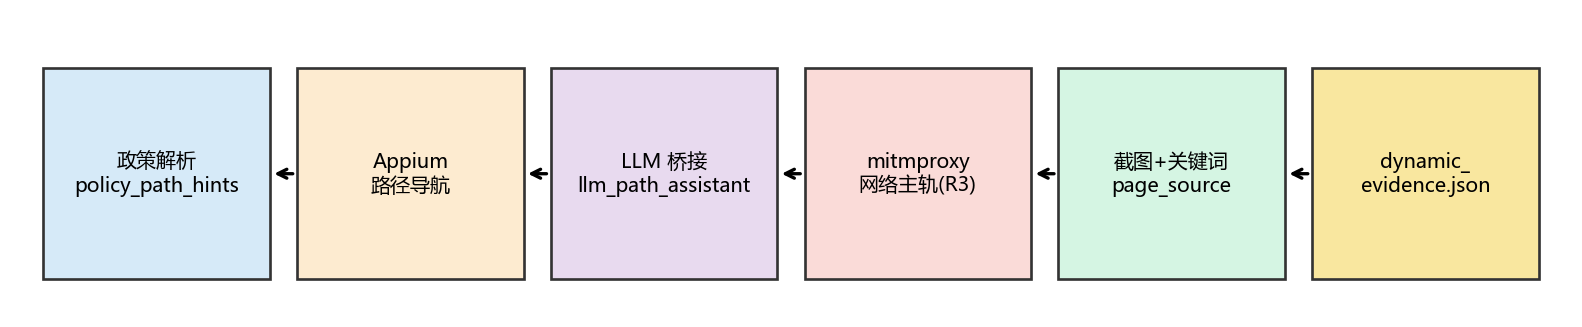
\includegraphics[width=0.98\linewidth]{fig_stage3_pipeline.png}
\end{frame}

\begin{frame}
    \frametitle{Lab4-2 实验管线（同意权 \textbullet\ mitm-primary）}
    \small
    \begin{enumerate}
        \item \textbf{Before}：\texttt{动态验证} + mitmproxy
        \item 真机操作：关闭隐私相关开关（或切换基本版等）
        \item \textbf{After}：同上
        \item \textbf{主判定}：比对关开关前后 mitm 流量中的 \textbf{Tracker} 与 \textbf{PII 网络字段}——关后仍传则同意权未生效。
        \item \textbf{辅助}：比对 Appium 页面 \textbf{关键词} 与 \textbf{导航点击}——关后 UI 是否仍暴露「个性化」等信号。
    \end{enumerate}
    \vspace{0.3em}
    \centering
    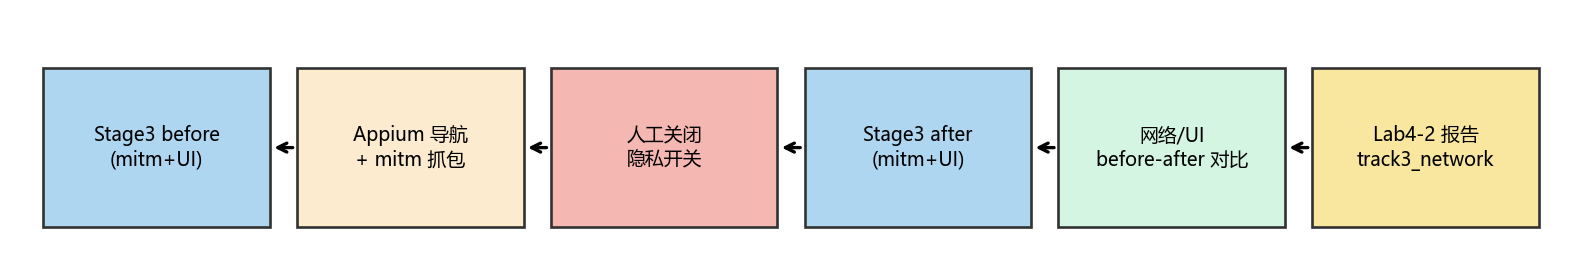
\includegraphics[width=0.92\linewidth]{fig_lab42_pipeline.png}
\end{frame}

\begin{frame}
    \frametitle{Lab4-3 实验管线（访问权）}
    \small
    \begin{enumerate}
        \item \textbf{三份输入}：隐私政策（声明了哪些 PII）、动态取证（Frida + mitm）、用户导出的个人信息副本。
        \item \textbf{运行时汇总}：合并 Frida 与 mitm 观测 \arrown{} 「实际采集/传输了哪些 PII」。
        \item \textbf{副本比对}：运行时字段是否在副本中可查；副本字段是否与政策声明一致（taxonomy 别名匹配 + 人工审核）。
    \end{enumerate}
    \vspace{0.3em}
    \centering
    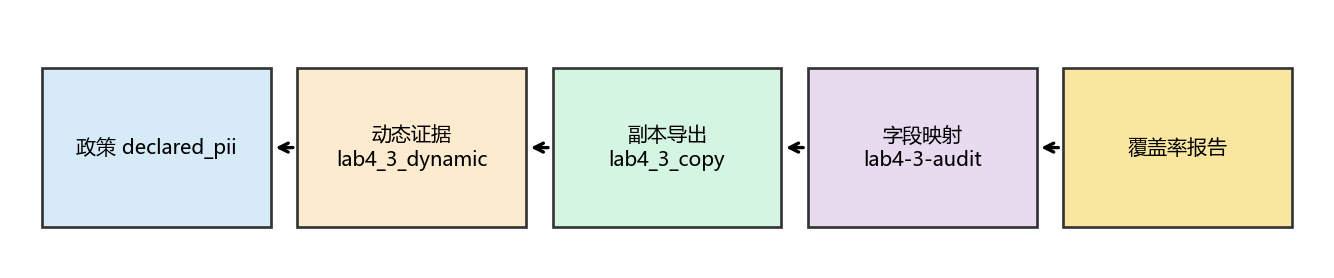
\includegraphics[width=0.88\linewidth]{fig_lab43_pipeline.png}
\end{frame}

\section{Frida 动态验证架构}

\begin{frame}
    \frametitle{Frida 一趟动态验证业务流程}
    \small
    \begin{tikzpicture}[
        node distance=0.55cm and 0.35cm,
        box/.style={draw, rounded corners=2pt, align=center, font=\scriptsize,
                    minimum width=2.1cm, minimum height=0.65cm},
        arr/.style={-{Stealth[length=2mm]}, thick}
    ]
        \node[box] (prep) {解析 \texttt{candidate\_pii}\\taxonomy + Stage2};
        \node[box, right=of prep] (conn) {端口 连接\\spawn / attach};
        \node[box, right=of conn] (load) {按序装载 Hook\\IMEI\arrown{}OkHttp\arrown{}PAPI};
        \node[box, below=of load] (grace) {Grace 窗口\\Appium 随机操作};
        \node[box, left=of grace] (ui) {Appium 导航\\截图 + 关键词};
        \node[box, left=of ui] (tail) {Tail 排空\\Reactor drain};
        \node[box, below=of ui] (out) {\texttt{frida\_result.events}\\写入 \texttt{dynamic\_evidence}};
        \draw[arr] (prep) -- (conn);
        \draw[arr] (conn) -- (load);
        \draw[arr] (load) -- (grace);
        \draw[arr] (grace) -- (ui);
        \draw[arr] (ui) -- (tail);
        \draw[arr] (tail) -- (out);
    \end{tikzpicture}
\end{frame}

\begin{frame}
    \frametitle{三层 Hook 设计与职责}
    \footnotesize
    \setlength{\tabcolsep}{3.5pt}
    \renewcommand{\arraystretch}{1.12}
    \begin{tabularx}{\linewidth}{|l|>{\raggedright\arraybackslash}p{1.9cm}|>{\raggedright\arraybackslash}X|>{\raggedright\arraybackslash}X|}
        \hline
        \textbf{Hook} & \textbf{脚本} & \textbf{职责} & \textbf{特点} \\
        \hline
        \textbf{IMEI\_HOOK} & \texttt{hook\_imei.js} &
        拦截 \texttt{TelephonyManager} 等设备标识符 API &
        \textbf{完全静态}：类/方法硬编码，不依赖混淆发现 \\
        \hline
        \textbf{OKHTTP\_HOOK} &
        \makecell[l]{\texttt{hook\_network\_}\\\texttt{okhttp.js}} &
        出站 HTTP 请求体/URL 污点；开/关权限前后比对 &
        源自 \textbf{rekit}；混淆感知枚举 \texttt{okhttp3.*} 指纹 \\
        \hline
        \textbf{PAPI\_HOOK} & \texttt{hook\_papi.js} &
        \texttt{api\_targets} 动态决定监测面 &
        \texttt{pii\_type} 分类；\texttt{stack\_summary} 调用栈节选 \\
        \hline
    \end{tabularx}
    \vspace{0.25em}
    \begin{itemize}\setlength{\itemsep}{0.12em}
        \item \textbf{装载顺序}：注册表 Hook（IMEI）\arrown{} OkHttp \arrown{} RPC 装载 PAPI（\texttt{installhooks}）
        \item \textbf{Lab4-2}：OkHttp 事件 + mitm 网络字段，开关前后污点对比
        \item \textbf{Lab4-3}：Frida 观测 $\cup$ mitm \texttt{pii\_key\_hits}，判断是否离设备上传
    \end{itemize}
\end{frame}

\begin{frame}
    \frametitle{Reactor：Frida 回调串行化}
    \small
    \begin{columns}[T]
        \column{0.48\textwidth}
        \textbf{问题}
        \begin{itemize}
            \item Frida 在独立线程投递 \texttt{script.on('message')}
            \item 多 Hook 并行回调直接写共享 \texttt{events{[]}} \arrown{} 竞态、丢事件
            \item 静态 Hook（IMEI）与动态 PAPI 同时触发时尤甚
        \end{itemize}
        \column{0.48\textwidth}
        \textbf{方案}
        \begin{itemize}
            \item \texttt{frida\_reactor.Reactor}：单 worker 线程 + 延迟队列
            \item 所有 \texttt{on\_message} 仅 \texttt{reactor.schedule(fn)}
            \item \texttt{stop(drain\_timeout=3s)}：停止前\textbf{排空}待处理回调
        \end{itemize}
    \end{columns}
    \vspace{0.5em}
    \centering
    \begin{tikzpicture}[
        box/.style={draw, rounded corners=2pt, align=center, font=\scriptsize, minimum height=0.7cm},
        arr/.style={-{Stealth[length=2mm]}, thick}
    ]
        \node[box, minimum width=2.2cm] (frida) {Frida 线程\\并发 \texttt{send()}};
        \node[box, minimum width=2.4cm, right=1.2cm of frida] (q) {Reactor 队列\\\texttt{schedule()}};
        \node[box, minimum width=2.2cm, right=1.2cm of q] (wk) {单线程 worker\\append event};
        \draw[arr] (frida) -- (q);
        \draw[arr] (q) -- (wk);
    \end{tikzpicture}
    \vspace{0.3em}
    \scriptsize
    配合 \texttt{wrap\_hook\_script}：\texttt{\_\_frida\_java\_install} 等待 \texttt{Java.available} 后再执行 Hook 体，避免 ART 未就绪时静态脚本失效。
\end{frame}

\section{Frida 工程卡点}

\begin{frame}
    \frametitle{Spawn vs Attach：核心困局}
    \small
    \begin{tabularx}{\textwidth}{|l|X|X|}
        \hline
        \textbf{模式} & \textbf{优势} & \textbf{本实验现状} \\
        \hline
        \textbf{Spawn}（冷启动暂停注入） & 可在 \texttt{resume} 前装完全部 Hook；可抓冷启动标识符读取 & \textbf{多数 App 不可用}：反注入、spawn 失败、MuMu 进程管理异常 \\
        \hline
        \textbf{Attach}（附着已运行进程） & 绕开部分 spawn 限制；与 Appium 共存较稳 & \textbf{默认 fallback}；\textbf{天然漏采}：注入前已发生的 API 调用无法回溯 \\
        \hline
    \end{tabularx}
    \vspace{0.4em}
    \begin{itemize}
        \item 策略：\texttt{spawn\_fallback\_attach=true}；Attach 后 \textbf{Grace}（默认 30s）+ \textbf{Tail}（60s）延长观测窗
        \item Appium 随机滑动/点击 + 网络发包，辅助在 MuMu 多进程中\textbf{锁定目标 PID}
    \end{itemize}
\end{frame}

\begin{frame}
    \frametitle{三类典型注入故障}
    \small
    \begin{tabularx}{\textwidth}{|l|X|l|}
        \hline
        \textbf{症状} & \textbf{机理} & \textbf{代表 App} \\
        \hline
        \texttt{java\_not\_ready} / \texttt{java\_timeout} & ART 未就绪或强防护阻塞 \texttt{Java.perform}；Hook 脚本无法进入 Java 桥 & \textbf{支付宝}（强反 Frida） \\
        \hline
        \texttt{No such process} & 进程在 attach/probe 窗口内被系统或 App 瞬杀；PID 失效 & \textbf{东方财富}、58同城 \\
        \hline
        MuMu \textbf{多进程 PID 混淆} & 包名对应多个进程，attach 到错误进程（WebView/推送子进程） & 智联招聘、小红书等 \\
        \hline
    \end{tabularx}
\end{frame}

\begin{frame}
    \frametitle{采集失败的三层漏斗}
    \footnotesize
    \centering
    \begin{tikzpicture}[
        level/.style={draw, rounded corners=3pt, align=center, font=\scriptsize,
                      text width=0.9\linewidth, inner sep=3pt, minimum height=0.62cm},
        arr/.style={-{Stealth[length=2mm]}, thick}
    ]
        \node[level, fill=red!12] (L1) {第 1 层：\textbf{Java 桥是否成功}？\\
            \texttt{java\_active} / \texttt{papi\_ready} / \texttt{java\_timeout}};
        \node[level, below=0.22cm of L1, fill=orange!15] (L2) {第 2 层：\textbf{目标 API 是否被调用}？\\
            导航未触发路径；Attach 漏采冷启动};
        \node[level, below=0.22cm of L2, fill=yellow!18] (L3) {第 3 层：\textbf{是否存在非 Hook 通讯路径}？\\
            原生 Socket、Cronet/QUIC、证书钉扎绕过代理};
        \draw[arr] (L1) -- (L2);
        \draw[arr] (L2) -- (L3);
    \end{tikzpicture}
    \vspace{0.25em}
    \begin{itemize}\setlength{\itemsep}{0.08em}
        \item 任一层失败 \arrown{} Frida 侧 \texttt{frida\_runtime\_events} 偏低或为空
        \item 本批 5 月主实验：6/9 App 的 Frida runtime 为 0；\textbf{mitm 网络轨}由此成为 Lab4-2/3 主证据
        \item PAPI 仍保留：对 tier1 App（小荷健康、世纪佳缘）补充 API 级 \texttt{stack\_summary}
    \end{itemize}
\end{frame}

\section{mitm 网络主轨}

\begin{frame}
    \frametitle{为何引入 mitm？}
    \small
    \begin{itemize}
        \item \textbf{OkHttp Hook 的局限}（即 rekit \texttt{okhttp.js} 路线）
        \begin{itemize}
            \item 仅覆盖 Java 层 OkHttp 栈；Native/Cronet/自研协议不可见
            \item Attach 漏采 + 混淆后类发现仍可能失败；与 Appium 同进程竞争
            \item Frida 不稳定时，Lab4-2 无法做可靠的开关前后污点对比
        \end{itemize}
        \item \textbf{mitm 的定位}：\textbf{进程无关}的全局 HTTP\texttt{(S)} 旁路抓包
        \begin{itemize}
            \item 替代 rekit OkHttp Hook 作为 Lab4-2/3 的\textbf{核心网络模块}
            \item Frida 降为辅助：PAPI 补 API 调用栈，IMEI Hook 补设备标识读取
        \end{itemize}   
    \end{itemize}
\end{frame}

\begin{frame}
    \frametitle{mitm 抓包与分析流程}
    \small
    \begin{enumerate}
        \item \textbf{设代理抓包}：MuMu 经 ADB 走 mitm 代理，Appium 导航期间持续记录 HTTP 流量。
        \item \textbf{离线分析}：扫描请求 URL/Body 中的 \textbf{PII 字段} 与 \textbf{Tracker 域名}（Umeng、Bugly、百度广告等）。
        \item \textbf{证据落盘}：输出流量条数、PII 命中、Tracker 命中，写入网络证据 JSON。
        \item \textbf{收尾}：清除代理，停止 mitm 进程。
    \end{enumerate}
    \vspace{0.3em}
    \scriptsize
    Lab4-2：开关前后各抓一趟，比对 Tracker / PII 是否仍传输 \sepbar
    Lab4-3：mitm 观测与 Frida 合并，判断运行时实际涉及哪些 PII
\end{frame}

\begin{frame}
    \frametitle{mitm 驱动的 Lab4-2 判定逻辑}
    \footnotesize
    \setlength{\tabcolsep}{3.5pt}
    \renewcommand{\arraystretch}{1.35}
    \begin{tabularx}{\linewidth}{|l|>{\raggedright\arraybackslash}X|>{\raggedright\arraybackslash}p{2.9cm}|}
        \hline
        \textbf{维度} & \textbf{含义} & \textbf{判定标签} \\
        \hline
        Tracker &
        关隐私开关后 SDK 仍向追踪域名发包 &
        \makecell[l]{\texttt{still\_transmitting\_}\\\texttt{after\_off}} \\
        \hline
        Tracker &
        开关有效，追踪传输停止 &
        \makecell[l]{\texttt{tracker\_stopped\_}\\\texttt{after\_off}} \\
        \hline
        PII 网络字段 &
        网络请求中 PII 字段不再出现 &
        \makecell[l]{\texttt{pii\_keys\_stopped\_}\\\texttt{after\_off}} \\
        \hline
        PII 网络字段 &
        关开关后仍上传个人信息字段 &
        \makecell[l]{\texttt{still\_leaking\_}\\\texttt{after\_off}} \\
        \hline
    \end{tabularx}
    \vspace{0.3em}
    \textbf{正面对照 --- Keep}：关后 \texttt{location}/\texttt{mac\_address} 等 PII 命中 0；Tracker 无泄漏。\\
    \textbf{风险案例 --- 钓鱼人}：Umeng、Bugly、百度广告关后仍传（82\arrown{}83 条流，6 个 Tracker 仍泄漏）。
\end{frame}

\begin{frame}
    \frametitle{mitm 实验结果（15 App \textbullet\ Lab4-2）}
    \centering
    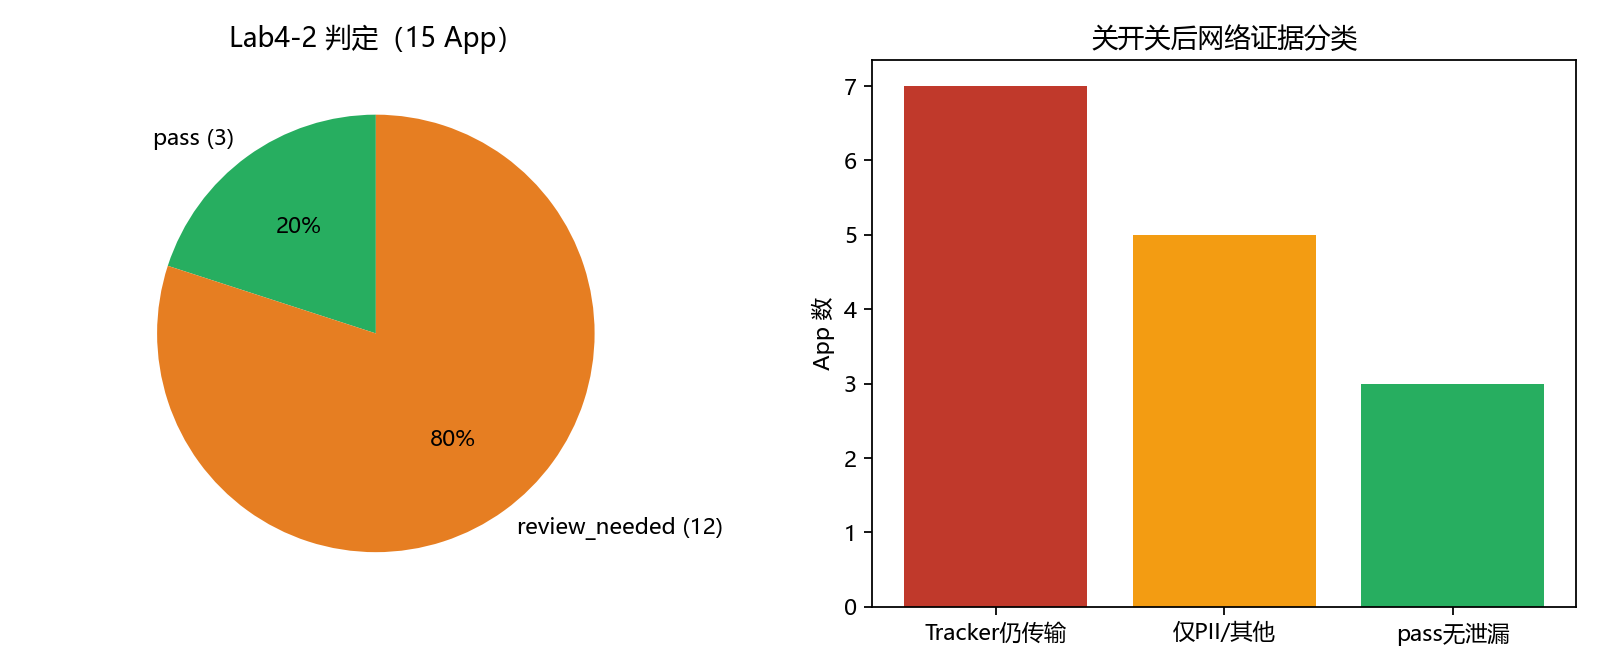
\includegraphics[width=0.45\linewidth]{fig_lab42_status.png}
    \hfill
    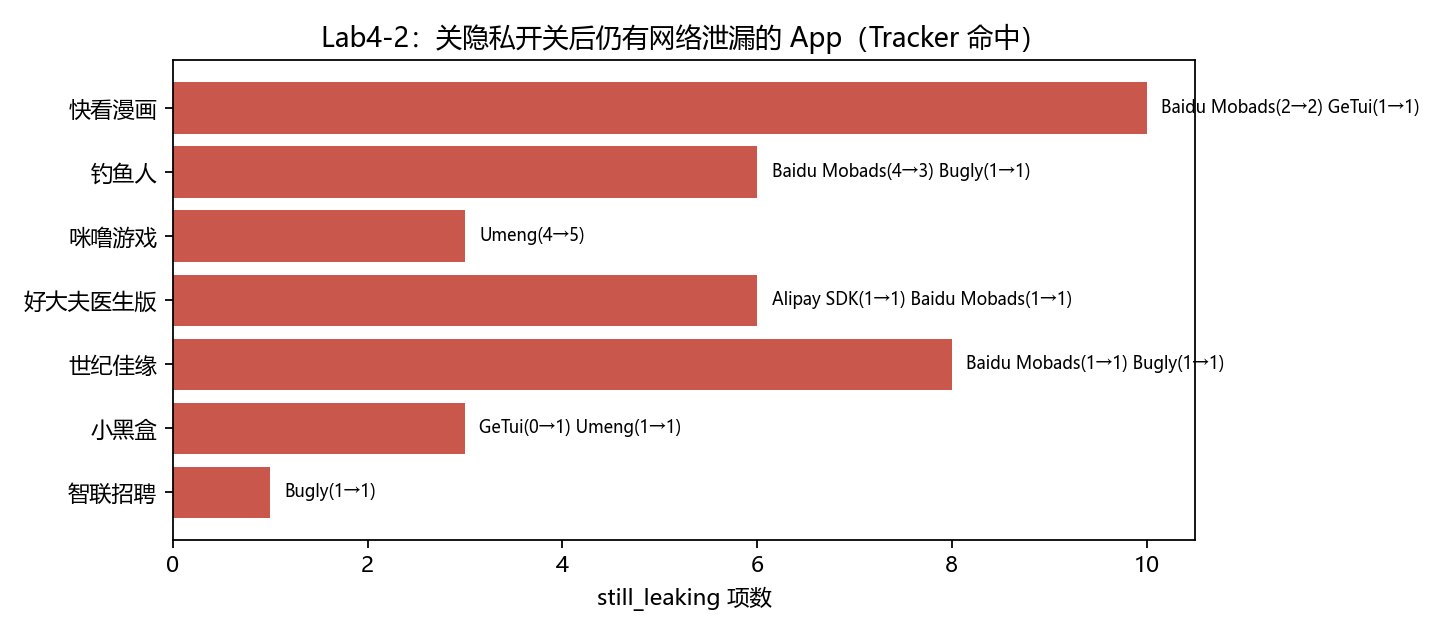
\includegraphics[width=0.48\linewidth]{fig_lab42_tracker_leaks.png}
    \vspace{0.3em}
    \scriptsize
    \begin{tabular}{lcccc}
        \toprule
        App & before 流 & after 流 & PII 命中 & 关后仍泄漏 \\
        \midrule
        小荷健康 & 272 & 312 & 58$\rightarrow$58 & 无 SDK Tracker；仍有 PII 传输 \\
        快看漫画 & 162 & 206 & 21$\rightarrow$17 & SDK Tracker（Umeng/百度/个推） \\
        世纪佳缘 & 234 & 276 & 38$\rightarrow$38 & SDK Tracker（百度/Bugly） \\
        钓鱼人 & 82 & 83 & 30$\rightarrow$33 & SDK Tracker（Umeng/Bugly/百度） \\
        Keep & 67 & 1 & 4$\rightarrow$0 & \textbf{否（pass）} \\
        \bottomrule
    \end{tabular}
\end{frame}

\begin{frame}
    \frametitle{mitm 在 Lab4-3 中的角色}
    \small
    \begin{itemize}
        \item \textbf{运行时观测合并}：\texttt{primary\_source} 多为 \texttt{mitm{+}frida}
        \begin{itemize}
            \item Frida：API 级（如 \texttt{clipboard}、\texttt{contact\_list}）+ \texttt{stack\_summary}
            \item mitm：离设备传输级（如 \texttt{account\_info}、\texttt{biometric\_info} 出现在请求体）
        \end{itemize}
        \item \textbf{污点完整性}：判断「采集到的 PII 是否经网络上送」---副本未含字段但 mitm 已命中 \arrown{} 访问权/透明度风险
        \item \textbf{局限}：证书痂皮 App 流量不入 mitm；HTTPS 解密依赖模拟器用户证书信任
    \end{itemize}
\end{frame}


\section{实验结果}

\begin{frame}
    \frametitle{Lab4-2 本批结果（15 App）}
    \centering
    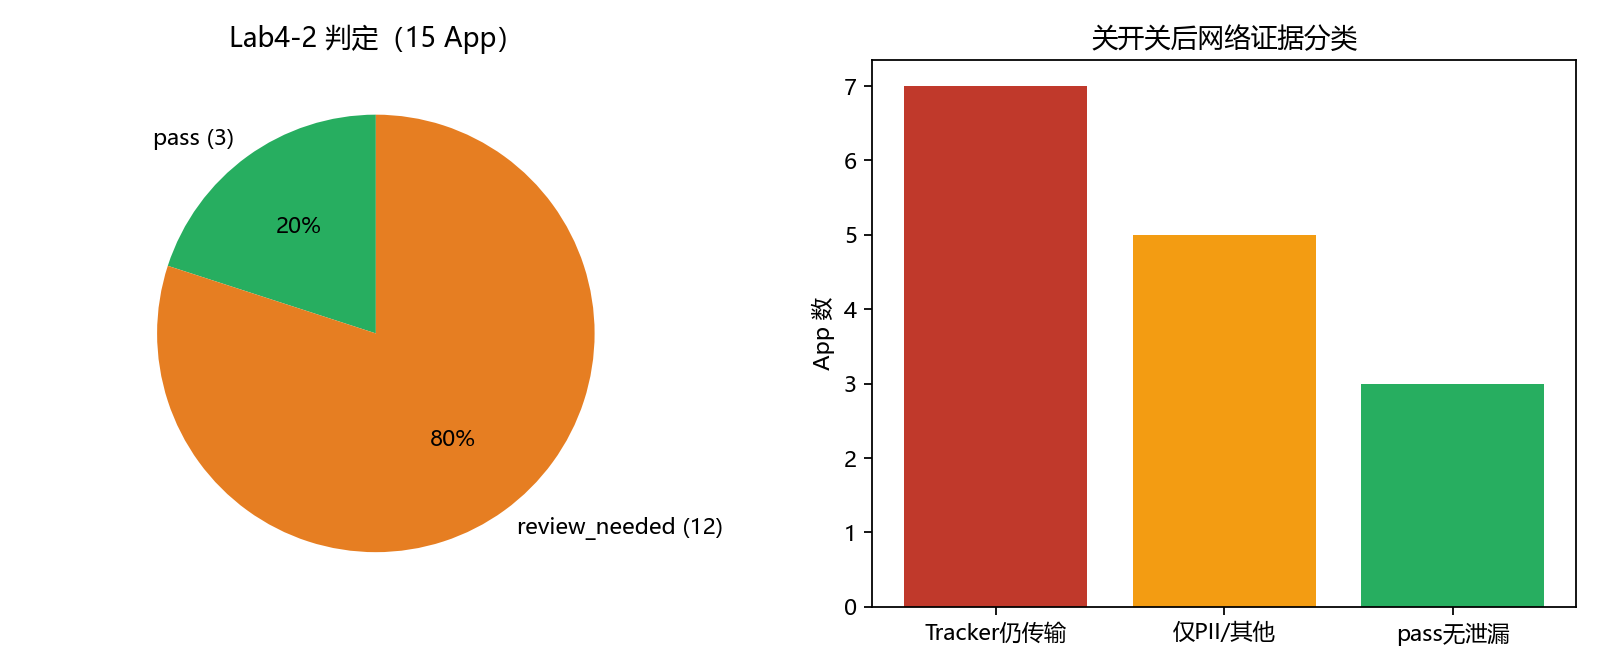
\includegraphics[width=0.45\linewidth]{fig_lab42_status.png}
    \hfill
    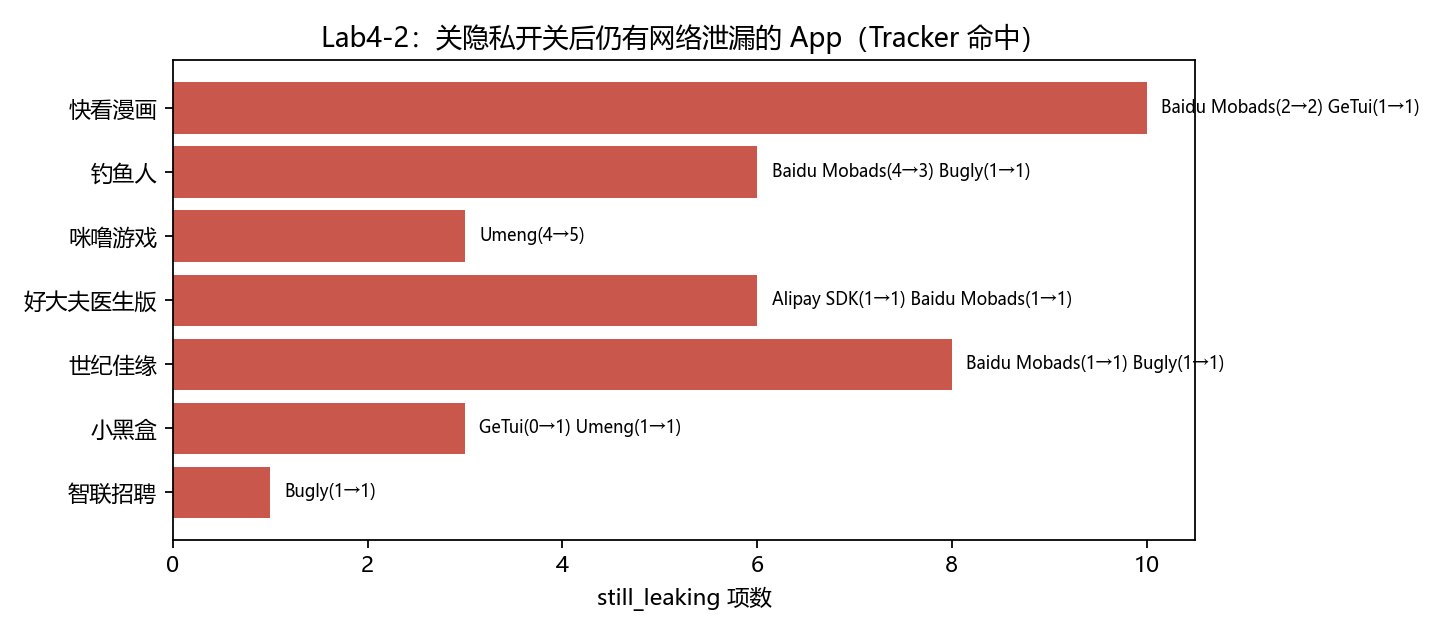
\includegraphics[width=0.48\linewidth]{fig_lab42_tracker_leaks.png}
    \vspace{0.3em}
    \scriptsize
    pass：Keep、支付宝、韭研公社 \sepbar 强案例：钓鱼人、好大夫、快看漫画、世纪佳缘
\end{frame}

\begin{frame}
    \frametitle{Lab4-2 网络流量 before/after}
    \centering
    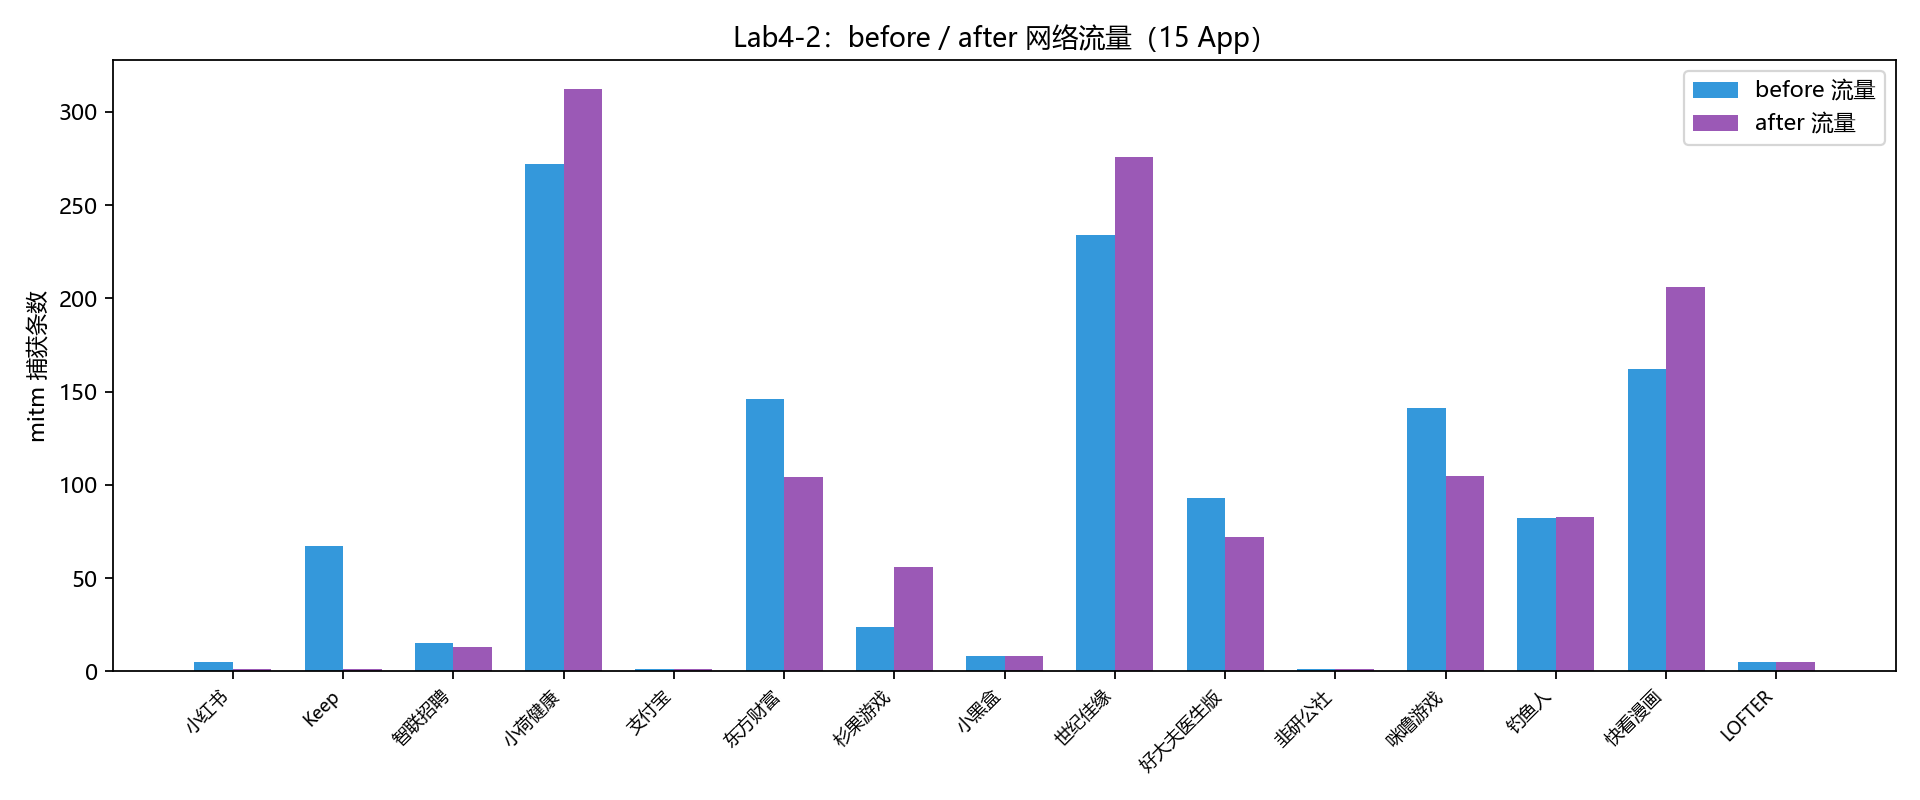
\includegraphics[width=0.95\linewidth]{fig_lab42_flows.png}
\end{frame}


\begin{frame}
    \frametitle{Lab4-3 人工审核结果（访问权）}
    \small
    \begin{tabularx}{\textwidth}{|l|X|}
        \hline
        \textbf{App} & \textbf{副本所含个人信息类型} \\
        \hline
        世纪佳缘 & 生物识别信息、手机号、账号/账户信息、身份信息 \\
        \hline
        小荷健康 & 手机号、账号/账户信息、身份信息 \\
        \hline
        智联招聘 & 手机号、身份信息、账号/账户信息、位置信息 \\
        \hline
        支付宝 & 手机号、身份信息 \\
        \hline
        东方财富 & 手机号、账号/账户信息、身份信息 \\
        \hline
    \end{tabularx}
    \vspace{0.5em}
    \centering
    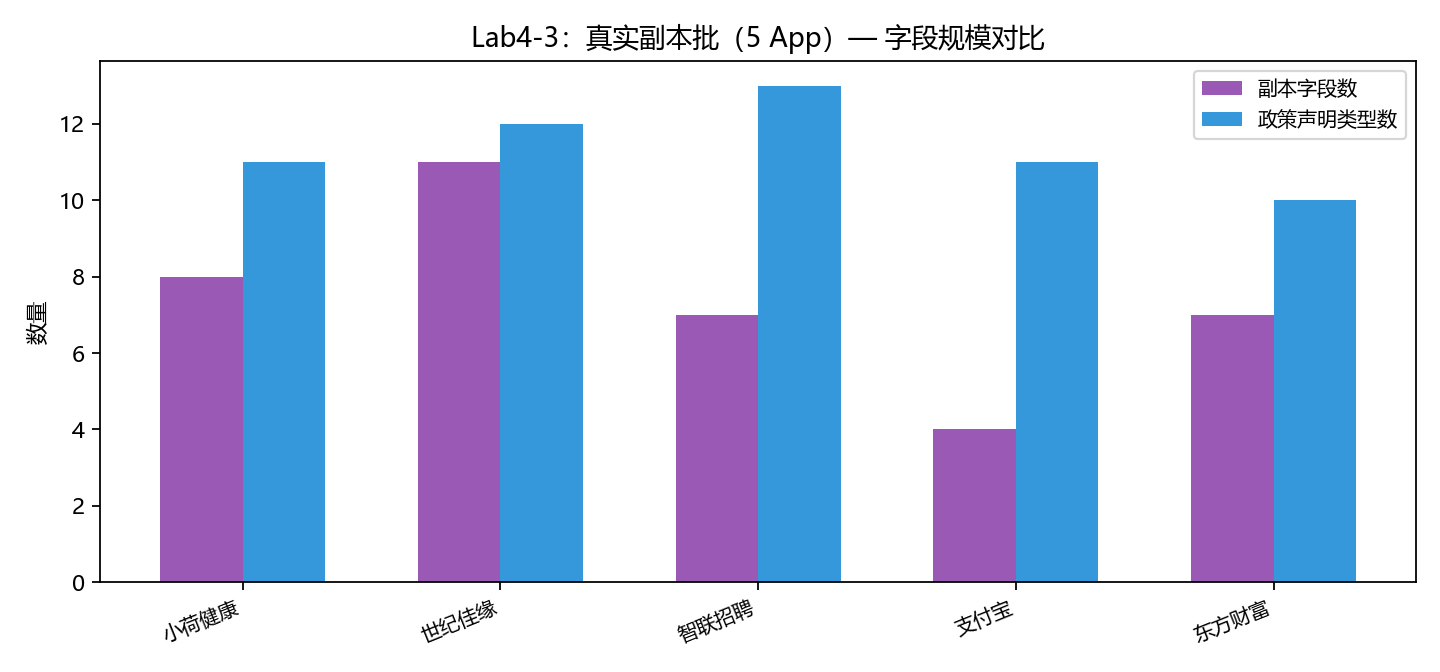
\includegraphics[width=0.82\linewidth]{fig_lab43_manual_results.png}
\end{frame}

\section{手段可用性总览}

\begin{frame}
    \frametitle{动态验证手段分工}
    \small
    \begin{tabularx}{\textwidth}{|l|X|X|}
        \hline
        \textbf{手段} & \textbf{强项} & \textbf{本批角色} \\
        \hline
        \textbf{Appium UI} & 政策路径导航、截图、关键词探测 & \textbf{主轨}：驱动隐私设置页到达 \\
        \hline
        \textbf{mitm 网络} & 全进程 HTTP 污点、Tracker 识别、开关前后对比 & \textbf{主轨}：Lab4-2/3 核心判定（\texttt{track3\_network}） \\
        \hline
        \textbf{Frida Hook} & API 级采集、调用栈、IMEI 精准 Hook & \textbf{辅助}：tier1 App 补 API 证据；受 Spawn/Attach 限制 \\
        \hline
        \textbf{静态 + KB} & APK 信号、法律知识库推断 & Lab4-1 知情权多源合并 \\
        \hline
    \end{tabularx}
\end{frame}

\section{总结与后续}

\begin{frame}
    \frametitle{后续工作}
    \small
    \begin{itemize}
        \item \textbf{Frida}：借鉴 \texttt{frida-tools} spawn gating；扩展 tier 探针（\texttt{probe\_hook.py}）；加固 PAPI \texttt{api\_targets}
        \item \textbf{mitm}：低流量 App 加长抓包窗口；证书钉扎绕过策略；补全 Lab4-3 剩余 6 款副本
        \item \textbf{UI}：支付宝 H5 容器 WebView context / OCR 辅助
        \item \textbf{taxonomy}：扩充副本字段别名，提升 Lab4-3 自动 \texttt{coverage\_rate}
    \end{itemize}
\end{frame}

\begin{frame}
    \centering
    \Huge 感谢聆听
\end{frame}

\end{document}
